\documentclass[spec, och, labwork]{SCWorks}
\usepackage{preamble}

\title{Теория псевдослучайных генераторов}
\author{Гущина Андрея Юрьевича} % Фамилия, имя, отчество в родительном падеже

\begin{document}
\selectlanguage{russian}
\chair{теоретических основ компьютерной безопасности и криптографии}
\course{4}
\group{431}
\department{факультета компьютерных наук и информационных технологий}
\napravlenie{10.05.01 "--- Компьютерная безопасность}

% Предмет для labwork2
% \subject{} 

% Для студентки. Для работы студента следующая команда не нужна.
% \studenttitle{Студентки}

% Заведующий кафедрой
% \chtitle{доцент} % степень, звание
% \chname{М.~Б.~Абросимов}

%Научный руководитель (для реферата преподаватель проверяющий работу)
\satitle{доцент} %должность, степень, звание
\saname{И.~И.~Слеповичев}

% Руководитель практики от организации (только для практики,
% для остальных типов работ не используется)
% \patitle{к.ф.-м.н.}
% \paname{С.~В.~Миронов}

% Семестр (только для практики, для остальных
% типов работ не используется)
%\term{8}

% Наименование практики (только для практики, для остальных
% типов работ не используется)
%\practtype{преддипломная}

% Продолжительность практики (количество недель) (только для практики,
% для остальных типов работ не используется)
%\duration{4}

% Даты начала и окончания практики (только для практики, для остальных
% типов работ не используется)
%\practStart{30.04.2019}
%\practFinish{27.05.2019}

% Год выполнения отчета
\date{\the\year{}}

\maketitle

% Включение нумерации рисунков, формул и таблиц по разделам
% (по умолчанию - нумерация сквозная)
% (допускается оба вида нумерации)
% \secNumbering

\tableofcontents

\section{Постановка задачи}

\subsection{Цель}
\begin{enumerate}
  \item Сгенерировать псевдослучайную последовательность заданным методом.
  \item Исследовать полученную псевдослучайную последовательность на случайность.
\end{enumerate}

\subsection{Исходные данные}
Исходными данными для лабораторных занятий являются метод генерации
псевдослучайных чисел, диапазон генерации случайных чисел, функция
распределения, которой должны подчиняться случайные числа, количество
генерируемых чисел.

В данной работе используются ППСЧ, сгенерированные с помощью программы,
разработанной в практическом задании №1. Для генераторов указаны следующие
параметры (эти параметры также можно найти в файле \texttt{lab/generate.sh}):
\begin{itemize}
  \item \texttt{/g:lc /f:rnd-lc.dat /i:31104,625,6571,23}
  \item \texttt{/g:add /f:rnd-add.dat /i:30000,24,55,79,134,213,\\
    347,560,907,1467,2374,3841,6215,10056,16271,26327,\\
    12598,8925,21523,448,21971,22419,14390,6809,21199,\\
    28008,19207,17215,6422,23637,59,23696,23755,17451,\\
    11206,28657,9863,8520,18383,26903,15286,12189,27475,\\
    9664,7139,16803,23942,10745,4687,15432,20119,5551,\\
    25670,1221,26891,28112,23779,17506}
  \item \texttt{/g:5p /f:rnd-5p.dat /i:19,7,13,17,19,\\
    1,0,1,0,1,1,0,0,1,0,1,0,1,1,0,0,1,1,1}
  \item \texttt{/g:lfsr /f:rnd-lfsr.dat /i:0,1,1,0,1,0,1,\\
    0,1,1,0,1,0,0,1,0,1,1,0,1,0,1,1,0,1,0,0,1,0,1,0,0,1,0,1,0}
  \item \texttt{/g:nfsr /f:rnd-nfsr.dat /i:0,1,1,0,1,0,1,0,\\
    1,1,0,1,0,0,1,0,1,1,0,1,0,1,1,0,1,0,0,1,0,1,0,0,1,0,1,0,\\
    19,2144512,412454,3124551}
  \item \texttt{/g:mt   /f:rnd-mt.dat   /i:1024,1234}
  \item \texttt{/g:rc4  /f:rnd-rc4.dat  /i:1,2,3,4,5,6,7,8,\\
    1,2,3,4,5,6,7,8,1,2,3,4,5,6,7,8,\\
    1,2,3,4,5,6,7,8,1,2,3,4,5,6,7,8,\\
    1,2,3,4,5,6,7,8,1,2,3,4,5,6,7,8,\\
    1,2,3,4,5,6,7,8,1,2,3,4,5,6,7,8,\\
    1,2,3,4,5,6,7,8,1,2,3,4,5,6,7,8,\\
    1,2,3,4,5,6,7,8,1,2,3,4,5,6,7,8,\\
    1,2,3,4,5,6,7,8,1,2,3,4,5,6,7,8,\\
    1,2,3,4,5,6,7,8,1,2,3,4,5,6,7,8,\\
    1,2,3,4,5,6,7,8,1,2,3,4,5,6,7,8,\\
    1,2,3,4,5,6,7,8,1,2,3,4,5,6,7,8,\\
    1,2,3,4,5,6,7,8,1,2,3,4,5,6,7,8,\\
    1,2,3,4,5,6,7,8,1,2,3,4,5,6,7,8,\\
    1,2,3,4,5,6,7,8,1,2,3,4,5,6,7,8,\\
    1,2,3,4,5,6,7,8,1,2,3,4,5,6,7,8,\\
    1,2,3,4,5,6,7,8,1,2,3,4,5,6,7,8,\\
    1,2,3,4,5,6,7,8}
  \item \texttt{/g:rsa  /f:rnd-rsa.dat  /i:39203,1024,17,14523}
  \item \texttt{/g:bbs  /f:rnd-bbs.dat  /i:312}
\end{itemize}


\section{Статистические свойства последовательности псевдослучайных чисел}

\subsection{Вычисление оценок}

\subsubsection{Линейный конгруэнтный метод}

\begin{itemize}
  \item Математическое ожидание = 0.4980023437500002
  \item Среднеквадратичное отклонение = 0.28966520307281585
  \item Относительная погрешность измерения математического ожидания для выборки из 5000 элементов: 0.642\%
  \item Относительная погрешность измерения среднеквадратичного отклонения для выборки из 5000 элементов: 0.048\%
\end{itemize}

\begin{figure}[H]
  \centering
  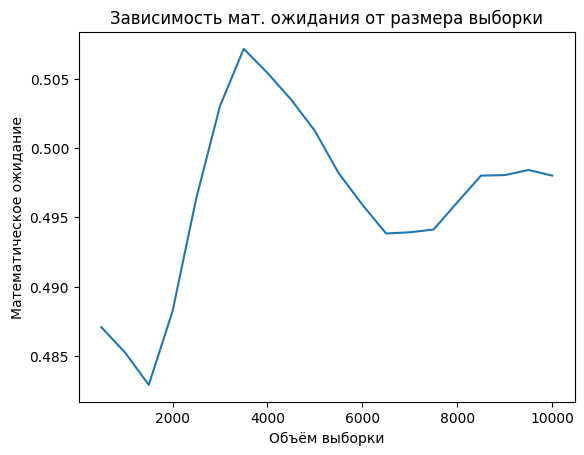
\includegraphics[width=0.9\textwidth]{lc_me}
\end{figure}
\begin{figure}[H]
  \centering
  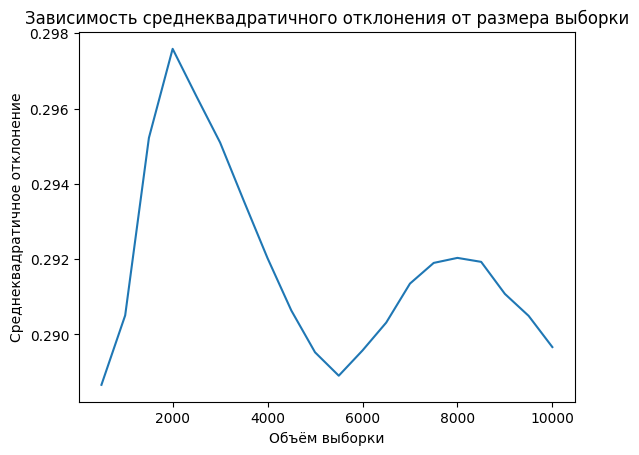
\includegraphics[width=0.9\textwidth]{lc_sd}
\end{figure}

\subsubsection{Аддитивный метод}

\begin{itemize}
  \item Математическое ожидание = 0.4959591796874994
  \item Среднеквадратичное отклонение = 0.2872104606725695
  \item Относительная погрешность измерения математического ожидания для выборки из 5000 элементов: 0.215\%
  \item Относительная погрешность измерения среднеквадратичного отклонения для выборки из 5000 элементов: 0.224\%
\end{itemize}

\begin{figure}[H]
  \centering
  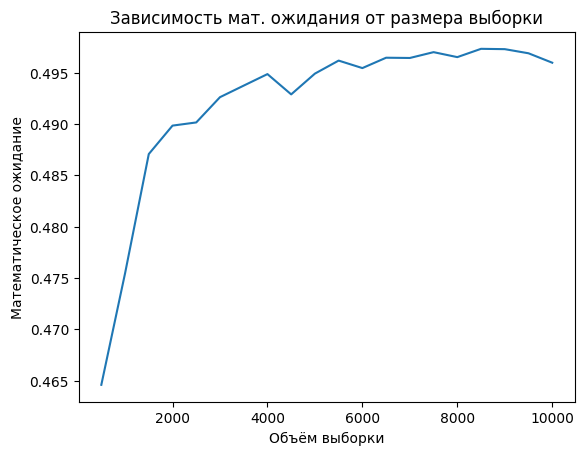
\includegraphics[width=0.9\textwidth]{add_me}
\end{figure}
\begin{figure}[H]
  \centering
  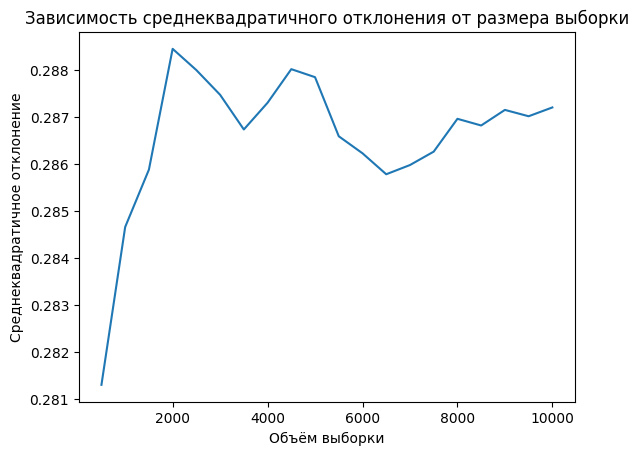
\includegraphics[width=0.9\textwidth]{add_sd}
\end{figure}

\subsubsection{Пятипараметрический метод}

\begin{itemize}
  \item Математическое ожидание = 0.49790820312500017
  \item Среднеквадратичное отклонение = 0.2899989510155476
  \item Относительная погрешность измерения математического ожидания для выборки из 5000 элементов: 0.409\%
  \item Относительная погрешность измерения среднеквадратичного отклонения для выборки из 5000 элементов: 0.003\%
\end{itemize}

\begin{figure}[H]
  \centering
  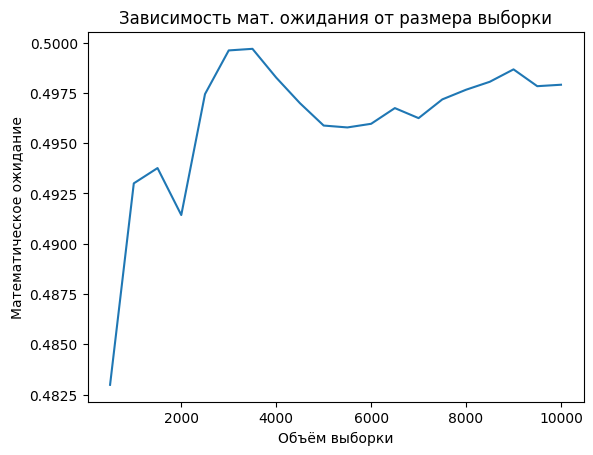
\includegraphics[width=0.9\textwidth]{5p_me}
\end{figure}
\begin{figure}[H]
  \centering
  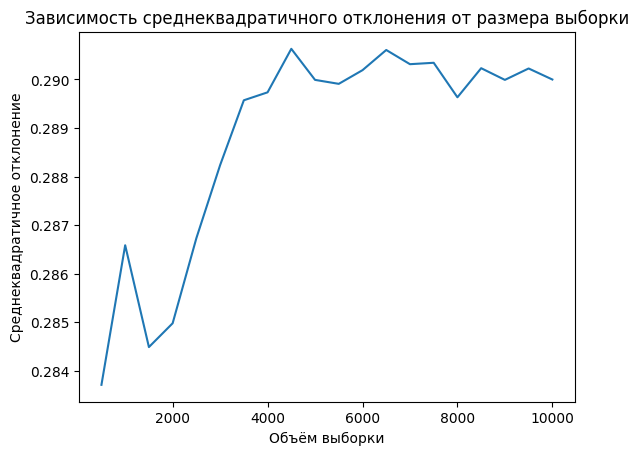
\includegraphics[width=0.9\textwidth]{5p_sd}
\end{figure}

\subsubsection{Регистр сдвига с обратной связью (РСЛОС)}

\begin{itemize}
  \item Математическое ожидание = 0.49532001953125054
  \item Среднеквадратичное отклонение = 0.29063739013628703
  \item Относительная погрешность измерения математического ожидания для выборки из 5000 элементов: 0.923\%
  \item Относительная погрешность измерения среднеквадратичного отклонения для выборки из 5000 элементов: 0.613\%
\end{itemize}

\begin{figure}[H]
  \centering
  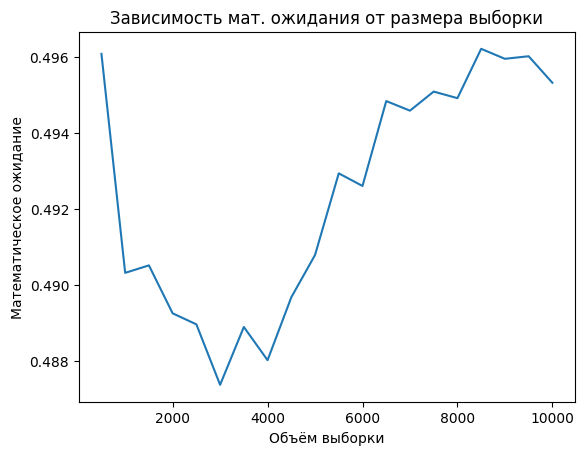
\includegraphics[width=0.9\textwidth]{lfsr_me}
\end{figure}
\begin{figure}[H]
  \centering
  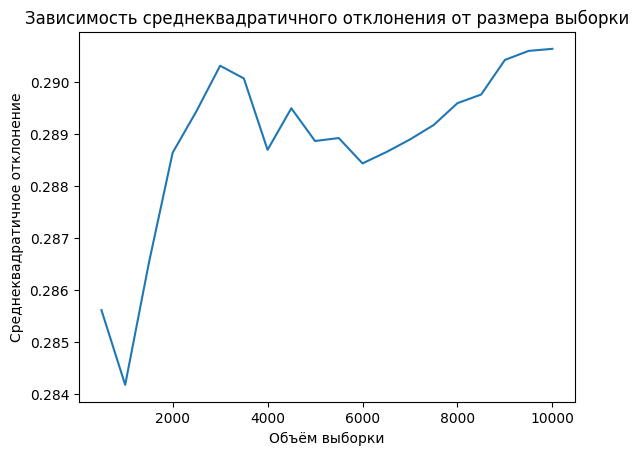
\includegraphics[width=0.9\textwidth]{lfsr_sd}
\end{figure}

\subsubsection{Нелинейная комбинация РСЛОС}

\begin{itemize}
  \item Математическое ожидание = 0.5033218749999994
  \item Среднеквадратичное отклонение = 0.29075993794219074
  \item Относительная погрешность измерения математического ожидания для выборки из 5000 элементов: 0.134\%
  \item Относительная погрешность измерения среднеквадратичного отклонения для выборки из 5000 элементов: 0.497\%
\end{itemize}

\begin{figure}[H]
  \centering
  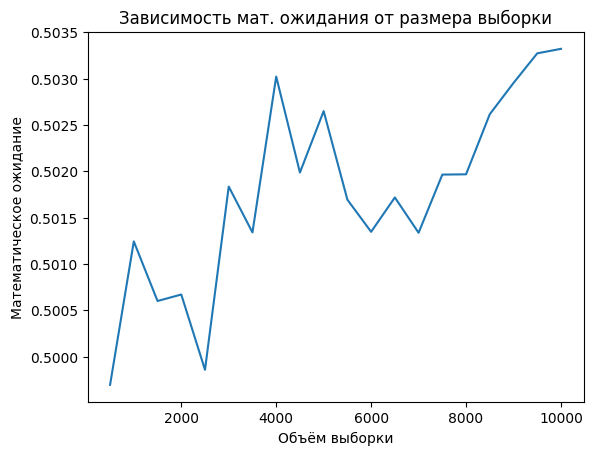
\includegraphics[width=0.9\textwidth]{nfsr_me}
\end{figure}
\begin{figure}[H]
  \centering
  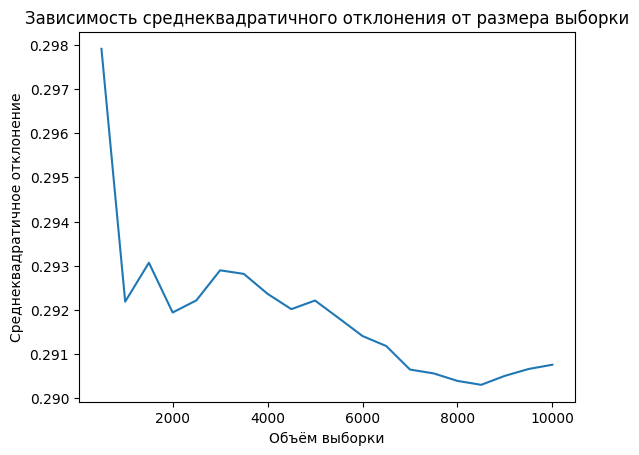
\includegraphics[width=0.9\textwidth]{nfsr_sd}
\end{figure}

\subsubsection{Вихрь Мерсенна}

\begin{itemize}
  \item Математическое ожидание = 0.4987525390624997
  \item Среднеквадратичное отклонение = 0.2883897385970719
  \item Относительная погрешность измерения математического ожидания для выборки из 5000 элементов: 0.643\%
  \item Относительная погрешность измерения среднеквадратичного отклонения для выборки из 5000 элементов: 0.469\%
\end{itemize}

\begin{figure}[H]
  \centering
  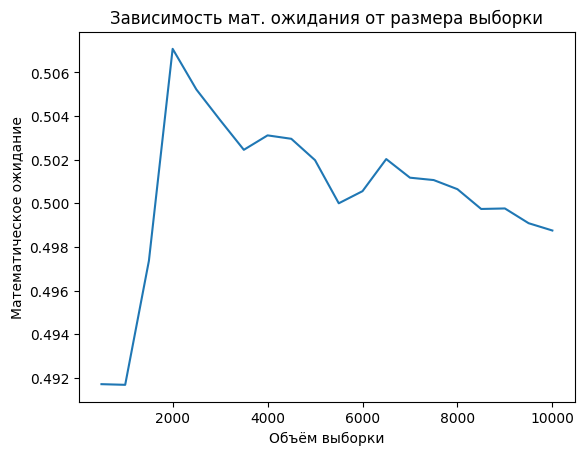
\includegraphics[width=0.9\textwidth]{mt_me}
\end{figure}
\begin{figure}[H]
  \centering
  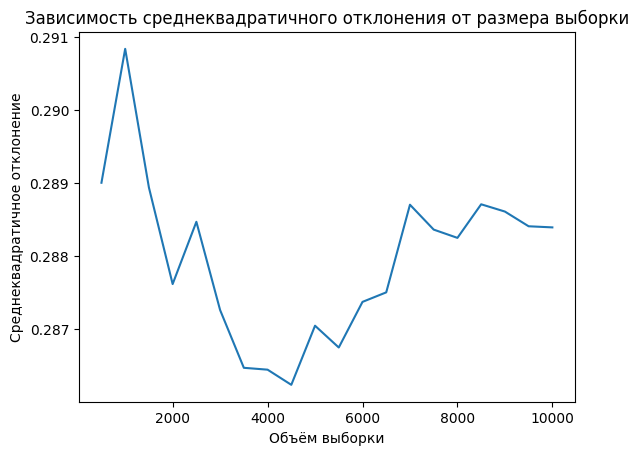
\includegraphics[width=0.9\textwidth]{mt_sd}
\end{figure}

\subsubsection{RC4}

\begin{itemize}
  \item Математическое ожидание = 0.12457070312500011
  \item Среднеквадратичное отклонение = 0.07160578956319438
  \item Относительная погрешность измерения математического ожидания для выборки из 5000 элементов: 0.29\%
  \item Относительная погрешность измерения среднеквадратичного отклонения для выборки из 5000 элементов: 0.003\%
\end{itemize}

\begin{figure}[H]
  \centering
  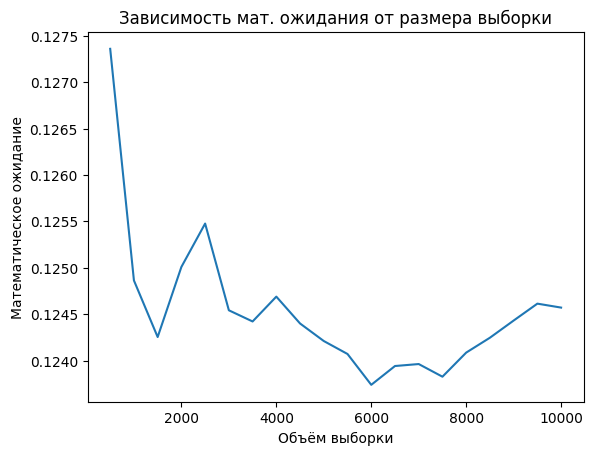
\includegraphics[width=0.9\textwidth]{rc4_me}
\end{figure}
\begin{figure}[H]
  \centering
  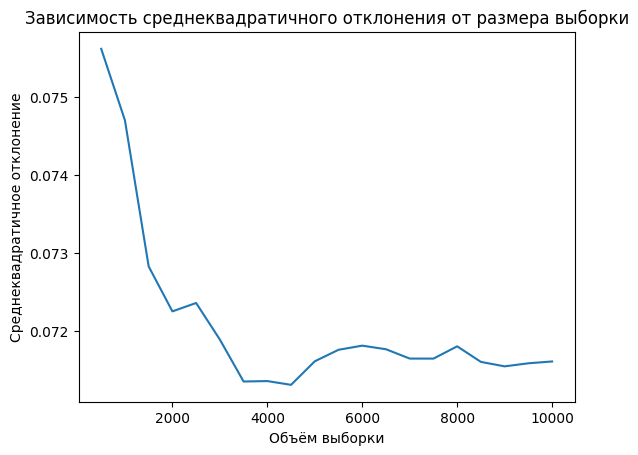
\includegraphics[width=0.9\textwidth]{rc4_sd}
\end{figure}

\subsubsection{ГПСЧ на основе RSA}

\begin{itemize}
  \item Математическое ожидание = 0.47569716796875
  \item Среднеквадратичное отклонение = 0.26404647855613683
  \item Относительная погрешность измерения математического ожидания для выборки из 5000 элементов: 0.012\%
  \item Относительная погрешность измерения среднеквадратичного отклонения для выборки из 5000 элементов: 0.01\%
\end{itemize}

\begin{figure}[H]
  \centering
  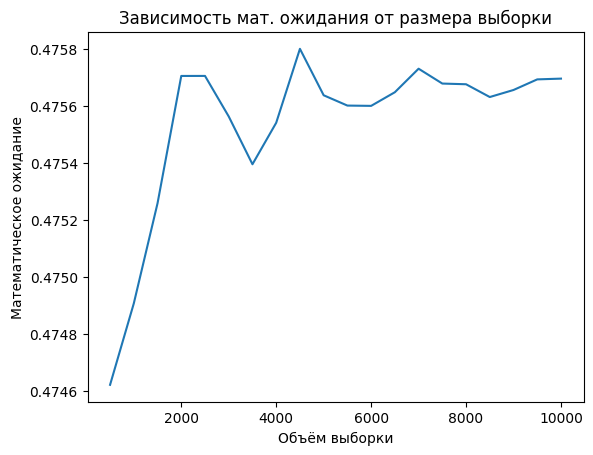
\includegraphics[width=0.9\textwidth]{rsa_me}
\end{figure}
\begin{figure}[H]
  \centering
  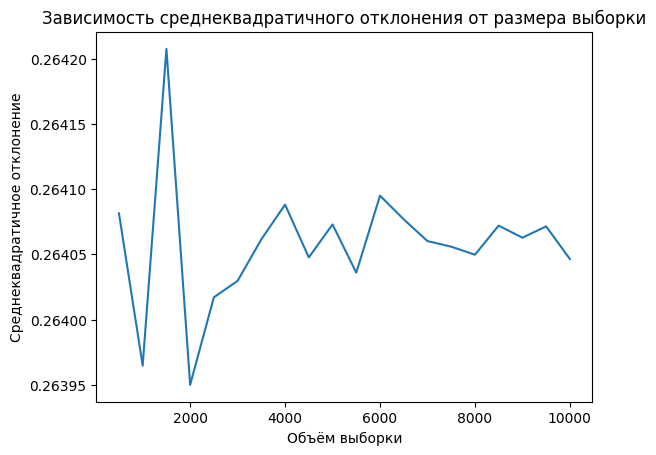
\includegraphics[width=0.9\textwidth]{rsa_sd}
\end{figure}

\subsubsection{Алгоритм Блюма-Блюма-Шуба}

\begin{itemize}
  \item Математическое ожидание = 0.005859765624999999
  \item Среднеквадратичное отклонение = 0.0036539883705292357
  \item Относительная погрешность измерения математического ожидания для выборки из 5000 элементов: 0.01\%
  \item Относительная погрешность измерения среднеквадратичного отклонения для выборки из 5000 элементов: 0.009\%
\end{itemize}

\begin{figure}[H]
  \centering
  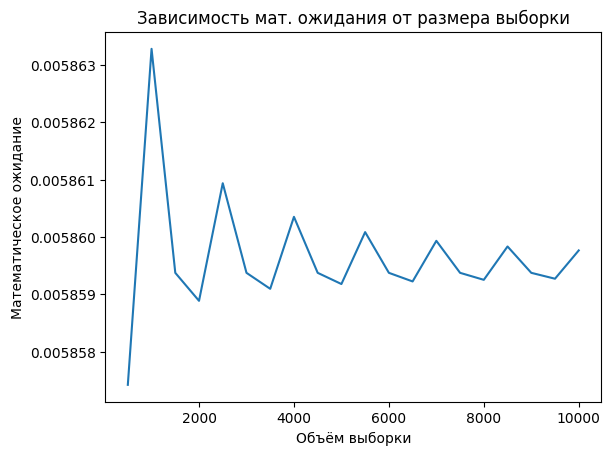
\includegraphics[width=0.9\textwidth]{bbs_me}
\end{figure}
\begin{figure}[H]
  \centering
  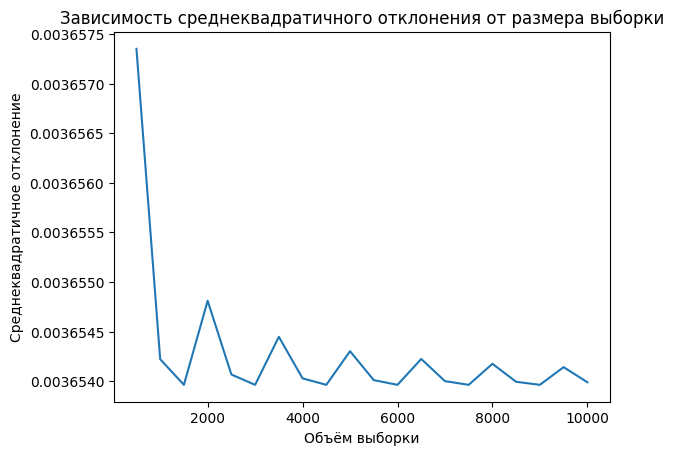
\includegraphics[width=0.9\textwidth]{bbs_sd}
\end{figure}

\subsection{Проверка критериев}

\begin{table}[H]
  \centering
  \footnotesize
  \begin{tabular}{|p{1.7cm}|c|c|c|c|c|c|c|}
    \hline
    ... & $\chi$-квадрат & Серий & Интервалов & Разбиений & Перестановок & Монотонности & Конфликтов \\ \hline
    Линейный конгруэнтный   & + & - & + & + & - & + & + \\ \hline
    Аддити"=вный            & + & + & + & + & + & + & + \\ \hline
    Пятипа"=раметрический   & + & + & + & + & + & + & + \\ \hline
    РСЛОС                   & + & + & + & + & + & - & + \\ \hline
    Нелинейная комб-я РСЛОС & + & - & + & - & - & - & + \\ \hline
    Вихрь Мерсенна          & + & + & + & + & + & + & + \\ \hline
    RC4                     & - & - & - & - & + & + & + \\ \hline
    RSA                     & - & - & + & - & - & - & - \\ \hline
    BBS                     & - & - & - & - & - & - & - \\ \hline
  \end{tabular}
\end{table}


\appendix

\section{Файл labwork.py}
\inputminted{python}{labwork.py}

\end{document}
